\documentclass{article}
% Language setting
% Replace `english' with e.g. `spanish' to change the document language
\usepackage[english]{babel}
\usepackage{graphicx}
\usepackage{listings}
\usepackage[colorlinks=true, allcolors=blue]{hyperref}
% Set page size and margins
% Replace `letterpaper' with `a4paper' for UK/EU standard size
\usepackage[letterpaper,top=2cm,bottom=2cm,left=3cm,right=3cm,marginparwidth=1.75cm]{geometry}
% Useful packages
\usepackage{amsmath}
\usepackage{graphicx}
\usepackage[colorlinks=true, allcolors=blue]

\title{Final Report}
\author{Team 2}

\begin{document}
\maketitle

\section{Introduction}

The intended user-base of our application, MyAudioEmailr, is professionals (e.g. senior executives), who typically receive large amounts of emails. In a professional context, staying apprised of emails is essential, because not doing so may result in missing important information. Keeping up with emails becomes more difficult the more emails there are to read. In a study of one software development company, Meyer et al. (2017: 1185) found that employees spent 14.5\% of their time reading emails. This means that, in terms of working time spent on tasks, reading emails was the second-ranked task, after developing (Meyer et al. 2017: 1188). Employees also reported feeling that time spent on emails was unproductive (Meyer et al. 2017). These findings suggest that email plays a large role in professional life, and too much time spent on email may negatively affect productivity. With these aspects in mind, it seems that traditional email clients, which rely solely on text-based communication, may not fully meet the needs of professionals. 


To meet the needs of professionals, MyAudioEmailr uses Text-to-Speech (TTS). Our application includes the functionalities common to email clients, meaning users can view their inbox, read, write and send emails. However, MyAudioEmailr can also read emails to the user, and the user can adjust the settings of speech, including speed, accent and scheduled reading time for their convenience. MyAudioEmailr is a web-based application. With this application, users can easily stay up to date with their emails, without having to review them manually. The goal of this application is to help professionals and other user types to save time, and help them to prioritise their work and lives more effectively.

\section{Project scope and objectives}
 The application aims to integrate text-to-speech technology into an email client, providing users with a convenient and easy way to interact with their emails, especially when they cannot or should not look at the screen, such as while driving or exercising. Additionally, MyAudioEmailr aims to provide high-quality and natural-sounding voice output by incorporating Google TTS API. The email interface is designed to be clean and intuitive for browsing and managing emails. The use of MySQL as the primary database system ensures the security and efficient storage and management of email data.

The project scope for MyAudioEmailr is to develop a user-friendly web application that integrates TTS technology into an email client. The application will allow users to access and manage their email accounts using both text and voice input and output. The application will have two main parts: email and TTS. The email part will be developed primarily in Java on the spec- and front-end, and MySQL on the back-end. The TTS part will be developed primarily in Python.


\section{Team profile}
\begin{enumerate}
  \item Georgia Gaffney; ggaffney2@sheffield.ac.uk
  \item Nana Kayamori; nkayamori1@sheffield.ac.uk
  \item Hok Yan Pun; hypun1@sheffield.ac.uk
  \item Baiyang Qu; Bqu5@sheffield.ac.uk
  \item Ziyu Wang; ZWang386@sheffield.ac.uk
  \item Mingqing Zhang; mzhang122@sheffield.ac.uk
\end{enumerate}
\underline{About the Gitlab:} The branch that ultimately saves all the code is the project branch, not the default doc branch. 
\\
\underline{Link to the video:}
\href{https://git.shefcompsci.org.uk/com6103-2022-23/team02/project/-/blob/project/video/MyAudioEmailr%20(Team%202).mp4}{Video}
\\
\underline{Link to the team Google drive:}
\href{https://drive.google.com/drive/folders/1L\_B7ax4ZjqrkdyzbJagLgAt-GhVxp-QS?usp=sharing}{Google Document}
\\
We have made our Google drive accessible to all staff at the University of Sheffield. However, please contact one of our team if there are any problems gaining access.

\section{Product backlog}
Backlog – A list of user stories that make up the complete product
The following are our user stories, as defined in our user stories map (link is provided in Appendix). The user stories are given in descending order of importance. The importance was determined by the priority of the requirements according to our client. 
 “As a user I want… :
\begin{itemize}
  \item Highest importance / core functionality:
  \begin{itemize}
    \item to access my account(s) using my email address(es) and password(s)
    \item to write and send emails to other accounts
    \item to receive emails from other accounts
    \item my incoming and outgoing emails to be automatically sorted into different folders - ‘inbox’ and ‘sent’
    \item to be able to explicitly choose an email to read
    \item to be able to explicitly choose an email to be read aloud
  \end{itemize}
  \item Medium importance:
   \begin{itemize}
   \item to see my inbox immediately once I log in
   \item to choose multiple emails to be read, one after the other
   \item to choose voices from a list that is varied by gender and accent
   \item to have all unread emails automatically read to me
   \item to have emails read to me by a specific time
   \item to be able to change the speed of dictation, in order to reduce the time needed to listen to emails
   \item to be able to have more than one email account/address
   \item to send/receive emails to/from different email providers
   \end{itemize}
    \item Low importance:
   \begin{itemize}
   \item spam emails to be automatically sorted into a dedicated ‘spam’ folder
   \item to be able to attach files to emails that I send
   \item to change the apparent emotion of a voice
   \item emails that have been written in Mandarin to be read in Mandarin
   \end{itemize}
\end{itemize}



\section{Analysis \& Design}
This part includes: System architecture, UML diagrams, Algorithm/Database design.
The project architecture is made up of two main parts: TTS and email functionality.

\subsection{Use case diagram}

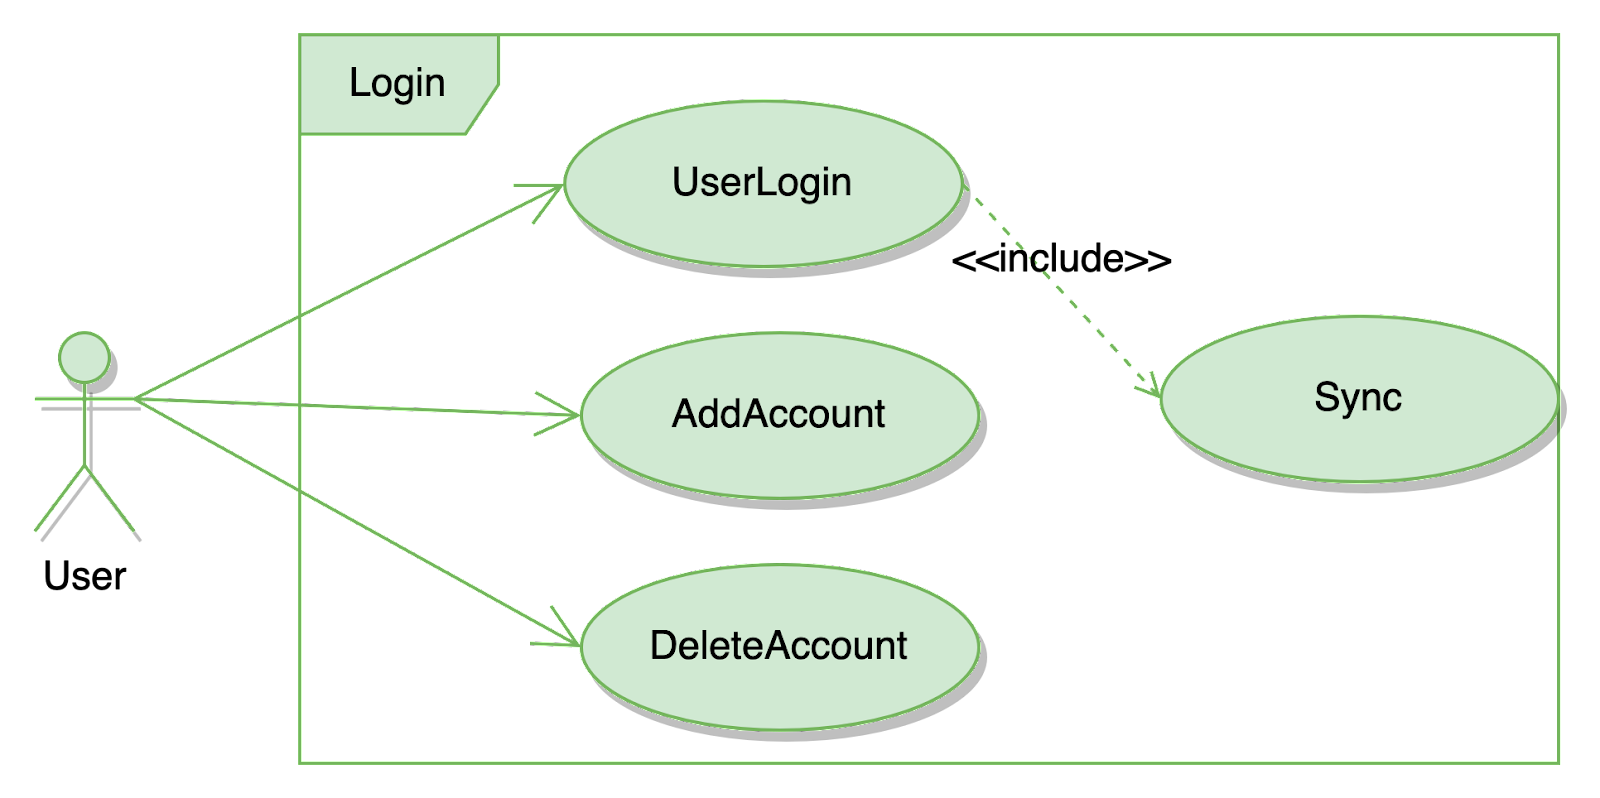
\includegraphics[width=0.8\textwidth]{UserCase_Login.png}
\begin{center}
Figure1: UseCase Login
\end{center}
You can view other class diagrams in the appendix.
\subsection{Sequence Diagram}
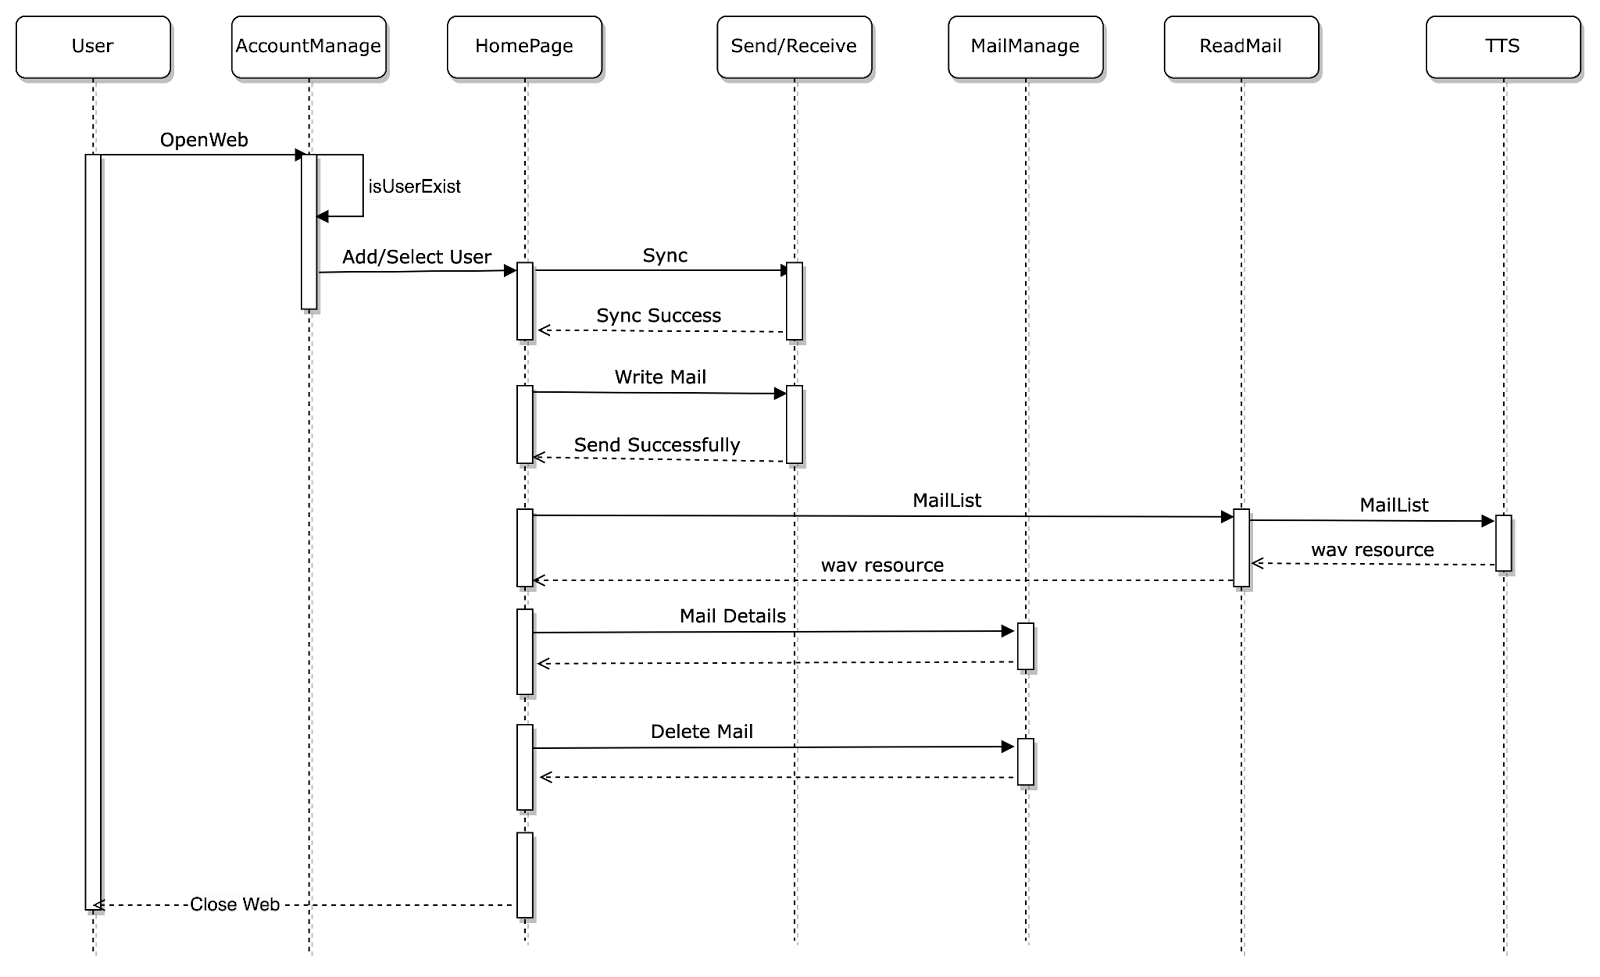
\includegraphics[width=1\textwidth]{SequenceDia.png}
\begin{center}
Figure2: SequenceDiag
\end{center}




\subsection{Text-to-Speech (TTS)}
The strategy of TTS we ultimately chose was an adaptation of Google’s text-to-speech API. Initially, we used concatenative speech synthesis. Concatenative speech synthesis uses a database of speech sounds, which are overlapped and added together to form words. We chose this strategy as it has historically been one of the most widely used TTS methods in the industry, and thus there are several reference texts concerning concatenative TTS (Jurafsky \& Martin, 2009). 

Although the large amount of available information on concatenation meant we could be well informed on the implementation of concatenative TTS, we encountered some issues with this strategy. Firstly, the resulting speech sounded inhuman, and the client raised this as a problem in the Week 8 meeting. The poor quality of the voice was due to discontinuities between diphones. Concatenative speech synthesis generally involves post-processing techniques to ensure the volume and pitch of the concatenated speech is relatively continuous, to the extent that joins are not perceptible (Jurafsky \& Martin, 2009). However, due to the time constraints of the project, we were unable to implement these techniques. Secondly, Requirement 5 stated: “The user shall have the ability to select the preferred voice from a list of 2-3”. When using concatenative speech synthesis, different voices are supported by recording different speakers pronouncing most of the diphones present in a language. However, we were only able to find a diphone dataset for one speaker.

Therefore, in order to address both the requirements and the client’s concerns, we needed to choose a different strategy for synthesis. We chose the Python library gTTS, which is an interface of Google's TTS API. Not only did this library provide improved quality, but it also offered multiple voices. The support of different voices allowed us to address Requirement 5. In fact, gTTS offers 7 accents for English, which we enabled in our application, as we erred on the side of giving the user more options of accents, not fewer.

We wrote two scripts in Python, using PyCharm, to handle the TTS functionality. The first is \texttt{text\_preprocessing.py}, which processes the email content and returns text. The second is \texttt{TTS.py}, which creates audio data using the external library gTTS and then processes the audio data. \texttt{TTS.py} is called by \texttt{httpHandler.py} (Section 6.2.7) and returns a path to a wav file.


\subsubsection{Text Processing}
This script takes an HTML file and turns it into a list of pronounceable words to pass to speech synthesis. There are 7 steps to process the text, hence 7 corresponding functions plus 1 pipeline function that calls all of them:
 \begin{itemize}
 \item \texttt{html2txt()}: takes an HTML file as the parameter, and turns it into plain text for processing using the Beautiful Soup module.
 \item \texttt{tokenize()}: breaks a text down to smaller, easier-to-process units. It takes a string; tokenizes the whole string using the \texttt{NLTK} library; and returns the whole text as a list of tokens.
 \item \texttt{strip()}: strips away useless parts from the tokenized text. It takes a list of tokens; removes punctuations that will not be converted into word representations for reading or used as markers in speech synthesis downstream; turns all remaining tokens lowercase; and returns a new complete list of tokens.
 \item \texttt{token\_parser()}: breaks down a token that is a concatenation of smaller tokens. It takes a list of tokens returned from the previous function; parses from beginning to end; keeps punctuation marks that will be used as markers in speech synthesis downstream; extracts alphabetical chunks and/or punctuations to be read along the scan; and concatenates “'s” to its preceding token as it is meant in the original message. The function then returns the list of tokens.
 \item \texttt{math\_parser()}: turns certain punctuation marks that were turned into word representations previously into a different word representation within a mathematical context. It takes a list within the list of lists; turns any “dash” or “dot” before a numeral into “minus” and “point” respectively; turns “asterix” between numerals into “times”, and “sir cum flex” (dictionary-pronounceable representation of “circumflex”) into “to the power of”; and concatenates numerals around any comma digit-separator. The function then returns the list of tokens with accurately (albeit not exhaustively) represented mathematical symbols if any.
 \item \texttt{num\_parser()}: turns numerals into their word representations. It takes a list within the list of lists; turns any sequence of number and ordinal suffix into an ordinal number, and all numbers into their word representations.
 \end{itemize}

Although the gTTS class implements text processing before synthesising speech, we found a number of benefits to using our own text processing. Benefits of using custom pre-processing include:

\begin{enumerate}
  \item Being able to parse html, using the Python library ‘Beautiful Soup’, which was necessary for the email-specific TTS task of MyAudioEmailr.
  \item Emails may contain textual elements such as links, and gTTS’ pre-processor occasionally leads to extensions such as ‘.ac’ being pronounced verbatim rather than spelled out. Due to our custom pre-processing, our synthesised speech spells out such extensions letter-by-letter, aiding listener understanding of links, internet addresses etc., which is essential for our demographic of professionals. As an example, gTTS’ text processing and our text processing system would handle the internet address “sheffield.ac.uk/” differently. While gTTS would pass the address directly to the synthesiser, our text processing first tokenises such strings, for example, the internet address would become: “sheffield dot ac dot uk slash”. Out-of-vocabulary/unusual tokens, such as ‘ac’, could then be pronounced letter-by-letter. In summary, using custom text-preprocessing allowed us to address issues not addressed by gTTS’ text-preprocessing. 
  \item Being able to retain exclamation marks for increased volume in the speech synthesis stage. This helps to better convey tone in emails. Therefore, the overall TTS system of our application could be better suited to email synthesis, specifically.
\end{enumerate}

\subsubsection{Prosody and Synthesis}
The \texttt{tts} function in the \texttt{TTS.py} script is primarily responsible for using the gTTS library to synthesise phrases, and then concatenating them, to create a complete utterance (i.e. a complete dictation of an email). It takes as parameters: wav\_name: a string that will be the name of the resulting wav file; email\_content: the HTML content of a given email as a string; accent, a string; and speed, a string, with the default of ‘normal’. The following is an example usage:

\begin{lstlisting}[language=Python]
speech = tts(wav_name='testus',
             email_content="""<p>Hello world!</p>""",
             accent='us',
             speed='fast')
\end{lstlisting}


There were two main reasons for using a single function for synthesis. Firstly, our application required that the synthesised speech be passed to the email part. If we were to use several functions to synthesise speech, we would need a ‘main’ function, that would be called by the email part, and call each of \texttt{TTS’} functions in turn. However, this may have slowed down processing, due to repeated function calls. A single function does not raise the same issues, as there is thus only one function call to pass speech to the email part. Secondly, it was necessary to use a \texttt{try… except…} structure to prevent the code from attempting to create empty speech objects (more information on this specific problem, and how we addressed it, is given below in this same section). In this instance, it was simpler to use the \texttt{try… except…} structure with a single function, as it meant that either speech or an error code would be returned to the email part. With these two reasons in mind, we decided that a single function should synthesise and return speech to the email part. It will now be explained why we used the gTTS library.

We have three main reasons for using gTTS: 
\begin{enumerate}
\item gTTS has comparably fewer dependencies than other Python libraries that perform TTS, such as ‘coqui-ai TTS’;  
\item it has wider platform support than another Python TTS library ‘espeak-ng’ (e.g. it can run easily on Apple OS);
\item finally, gTTS allows for speech data to be returned as an object, unlike libraries such as ‘pyttsx3’. As speech can be captured in a variable as byte data, gTTS enables post-processing of speech. We were able to take advantage of this by processing speech on the phrase-level, rather than on the entire email contents simultaneously. More detail on what phrases are in this context, and how \texttt{tts} processes them, are given below.
\end{enumerate}


A phrase, in the context of our application, is defined as text between certain delimiters, which are: “.,!?”. For example, given the HTML input string: 

\begin{lstlisting}
"""<p>The sun was setting; the sky was painted in shades of 
orange, pink, and purple.</p>"""
\end{lstlisting}

The phrases would be:
\begin{lstlisting}
the sun was setting the sky was painted in shades of orange , 
 pink , 
 and purple . 
\end{lstlisting}


Each phrase is shown on a new line, having been split by the delimiters. Synthesising the speech on a phrase-by-phrase basis allowed for more control of the output than would be allowed by synthesising the entire email contents at once. For example, after converting byte data to float64 arrays, it is possible to increase the volume of phrases ending in an exclamation mark, by simply multiplying the array elements by 2. However, there are a number of steps executed by the \texttt{tts} function, before synthesising the phrases.

The first step executed by \texttt{tts} is to check whether the user input for the accent parameter is supported. This check is achieved by using a list containing all of the supported accents as strings. If the input is not in this list, an exception is raised and the function is exited. \texttt{TTS.py} imports \texttt{text\_preprocessing.py}, meaning that it can call the pipeline \texttt{text\_proc}  function to process the email contents into a form that can be synthesised. 

Next, a \texttt{try… except…} block is opened. This structure is necessary because there are phrases which contain no alphanumeric characters. Passing such a phrase to the gTTS class while break the code and throw \texttt{AssertionError: No text to send to TTS API}. However, this error is not visible to the user on the front-end. Without a check, nothing would be played nor shown to the user, with no explanation. Although we implement text-preprocessing, accounting for all possible characters is not feasible, and thus we need a catch on the synthesis end, in case any non-synthesizable strings elude text-preprocessing. Therefore, if such strings are encountered during synthesis, our first method to avoid this problem is to return an error code -1 to \texttt{httpHandler.py}. This error code can then be passed to the email part so that an error can be shown to the user. This is more meaningful to the user than no sound playing, with no explanation given.

The second method is implemented within the \texttt{for} loop that is called on each phrase in the processed text. Speech data for each phrase are collected as arrays in a list. Once this \texttt{for} loop is entered, there is an \texttt{if… else…} structure that appends an array of zeros to the list in place of speech data, if the phrase has no alphanumeric characters. Such a phrase can thus be pronounced as silence. In such cases, the sampling rate, which is declared as variable \texttt{fs} above the \texttt{for} loop, is set as 24,000 Hz, to make it compatible with the gTTS speech data of the same sampling rate. If a phrase does contain alphanumeric characters, then it is handled by the \texttt{else} block. The phrase and selected accent are passed to the gTTS class, and the resulting speech data are converted from bytes to float64 encoding through the use of a buffer and the Soundfile library, which also returns the sampling rate. The speech data are then trimmed of silence to varying degrees, depending on punctuation. For example, the trailing silence of a phrase ending in a full-stop is left longer than that of a phrase ending in a comma. Once all arrays have been appended to the list, it is concatenated as a single array. The speed of this array can then be shifted up or down, if the user has selected a speed change. This is achieved by either increasing or decreasing the sampling rate, respectively. Soundfile is used to write all speech data for a given email to a wav file. Finally, a path to the created wav is returned when \texttt{tts} is called by \texttt{httpHandler.py}.

\section{Email Functionality}
\subsection{Technology selection}
\begin{itemize}
    \item Backend: SpringBoot, SpringShell
    \item Frontend: Thymeleaf, Bootstrap, JavaScript
    \item Database: MySQL
    \item Mail Framework: JavaMail
\end{itemize}
The reasons we chose these tools are as follows:

We chose SpringBoot as the backend technology because of its ease of use and development speed. SpringBoot provides a range of pre-configured features that simplifies the setup of new projects. It also has a large and active community that provides support and frequent updates, making it a reliable choice for building scalable and maintainable web applications.

MySQL was chosen as the database because it is open-source, scalable, and reliable. It is widely used and has a large community that provides support and resources, making it a safe and well-established choice for data storage.

JavaMail is a Java API used to send and receive email via SMTP, POP3, and IMAP. It provides a platform-independent and protocol-independent framework to build Java-based email client applications. JavaMail includes classes for handling attachments, forwarding, reply, HTML messages etc. It is widely used in enterprise applications and provides a flexible and powerful solution for email communication.

Lastly, we use SpringShell so that \texttt{TTS} developers do not need to perform additional configurations. Developers only need to install \texttt{Java JDK} and run the \texttt{Jar} file directly through the command line to conduct integration testing in the early stages.

Overall, our tool selections were made based on their ease of use, flexibility, reliability, and community support, among other factors. Information on Thymeleaf and Bootstrap Will be given in Section 6.2.8, as such information concerns the frontend.

\subsection{Function Details}
\subsubsection{Login}
When a user logs into the system, the system checks if a \texttt{deviceId} is stored in the cookie. It is a string composed of "current time - 6 random letters" that is almost impossible to duplicate. If the \texttt{deviceId} is detected, the system will query the accounts in the database for a match and display the \texttt{SelectAccount} page. If not, the login page is displayed.

Additionally, the system automatically sends a request to the \texttt{IMAPserver} on every login to obtain the latest emails and stores them in the system's database. \\
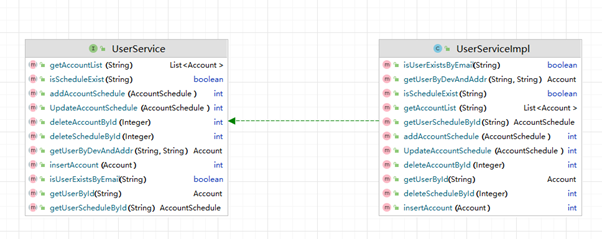
\includegraphics[width=0.8\textwidth]{UserService.png}
\begin{center}
Figure4: SequenceDiag
\end{center}

\subsubsection{Reading mails}
When a user requests to read a single email, the system will directly send the email to the TTS part and wait for the conversion to complete. This function is lacking, as once the function is triggered, the user cannot determine the current progress of the email conversion.

Both "reading some specific emails" and "reading all unread emails" functions use Socket. The logic for triggering these two functions by clicking buttons or through scheduled tasks is the same, the only difference being whether they are triggered by a timed task.\\
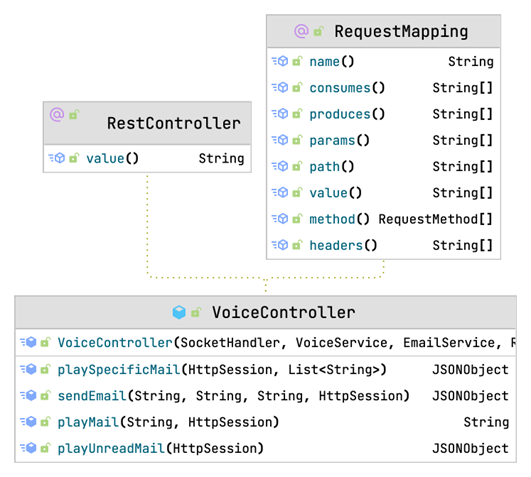
\includegraphics[width=0.5\textwidth]{VoiceController.png}
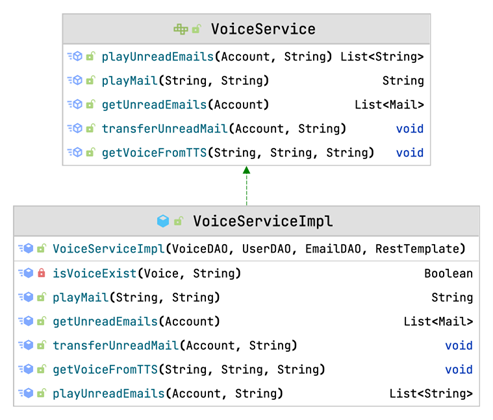
\includegraphics[width=0.5\textwidth]{VoiceService.png}
\begin{center}
Figure5: VoiceController\hspace{6cm}Figure6:VoiceService
\end{center}

\subsubsection{Send \& Receive Mails}
Upon successful login, the user is automatically redirected to the inbox page, where they can easily view, delete, and read all the emails that are currently present in their inbox. The backend component of the system is responsible for synchronising email data every ten minutes, and users can also manually synchronise their email information by clicking on the "Sync" button on the top right of the page. By clicking on the "details" button, users can view email details, including email text.

When a user decides to read an email, the system sends a request to the \texttt{TTS} module, which then processes the request and generates an audio file based on the email content. The \texttt{TTS} module subsequently sends the audio file information to the email system, which stores it in the database and sends the email information (i.e., the generated file path) to the frontend via a socket. The frontend listens for this event and displays a pop-up window that allows the user to play the audio of the email content.

To send emails, the system uses the Simple Mail Transfer Protocol (SMTP), which can be done by clicking on the "write message" menu.\\
\begin{center}
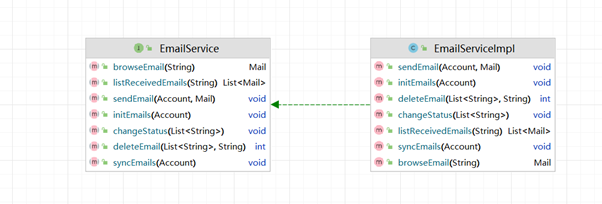
\includegraphics[width=0.7\textwidth]{EmailService.png}
\end{center}
\begin{center}
Figure7: EmailService
\end{center}

\subsubsection{SocketHandler}
\begin{center}
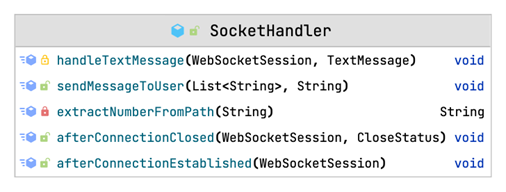
\includegraphics[width=0.4\textwidth]{SocketHandler.png}
\end{center}
\begin{center}
Figure8: SocketHandler
\end{center}
\texttt{SocketHandler} handles socket requests. When users need to read multiple emails, each email converted to speech will be sent one by one in order. This way, we can avoid users waiting too long for emails to be read.

\subsubsection{SMTP and IMAPHandler}
These two classes are used to send requests to SMTP and IMAP servers. 
The IMAP server is used to receive emails. \texttt{IMAPHandler} converts Message and \texttt{MimeMessage} objects from the server to an \texttt{ArrayList<Mail>} type and returns them. 
\texttt{SMTPHandler} converts \texttt{Mail} type objects to \texttt{MimeMessage} type and sends them to the server.
\begin{center}
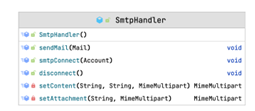
\includegraphics[width=0.3\textwidth]{smtpHandler.png} 
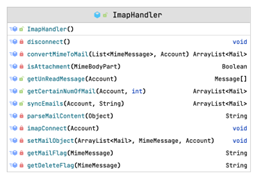
\includegraphics[width=0.3\textwidth]{imapHandler.png}
\end{center}
\begin{center}
Figure9: SmtpHandler and ImapHandler
\end{center}
\subsubsection{Settings}
 On the 'Settings' page, users can configure their account settings, such as the voice accent. MyAudioEmailr only supports English, for which there are the following accents: Australia, United Kingdom, United States, Canada, India, Ireland, and South Africa. Users can also set the time for scheduled email reading on this page. Once a scheduling is saved, the system will automatically convert and play the emails as speech at the selected time every day.

The scheduled tasks consist of reading all unread emails at a specific time, initiating the conversion of emails to speech at a particular time, and background checking for new emails. Since each task is user-specific, we cannot use the @Scheduled annotation in Spring Boot to automatically start them during development. Therefore, we implement Runnable to write the scheduled tasks and use cron expressions to set the trigger time.

To improve the efficiency and speed of email to speech conversion, the backend will start TTS one hour in advance of the scheduled time. This will ensure, in most cases, that the speech files are ready by the selected time.
\begin{center}
    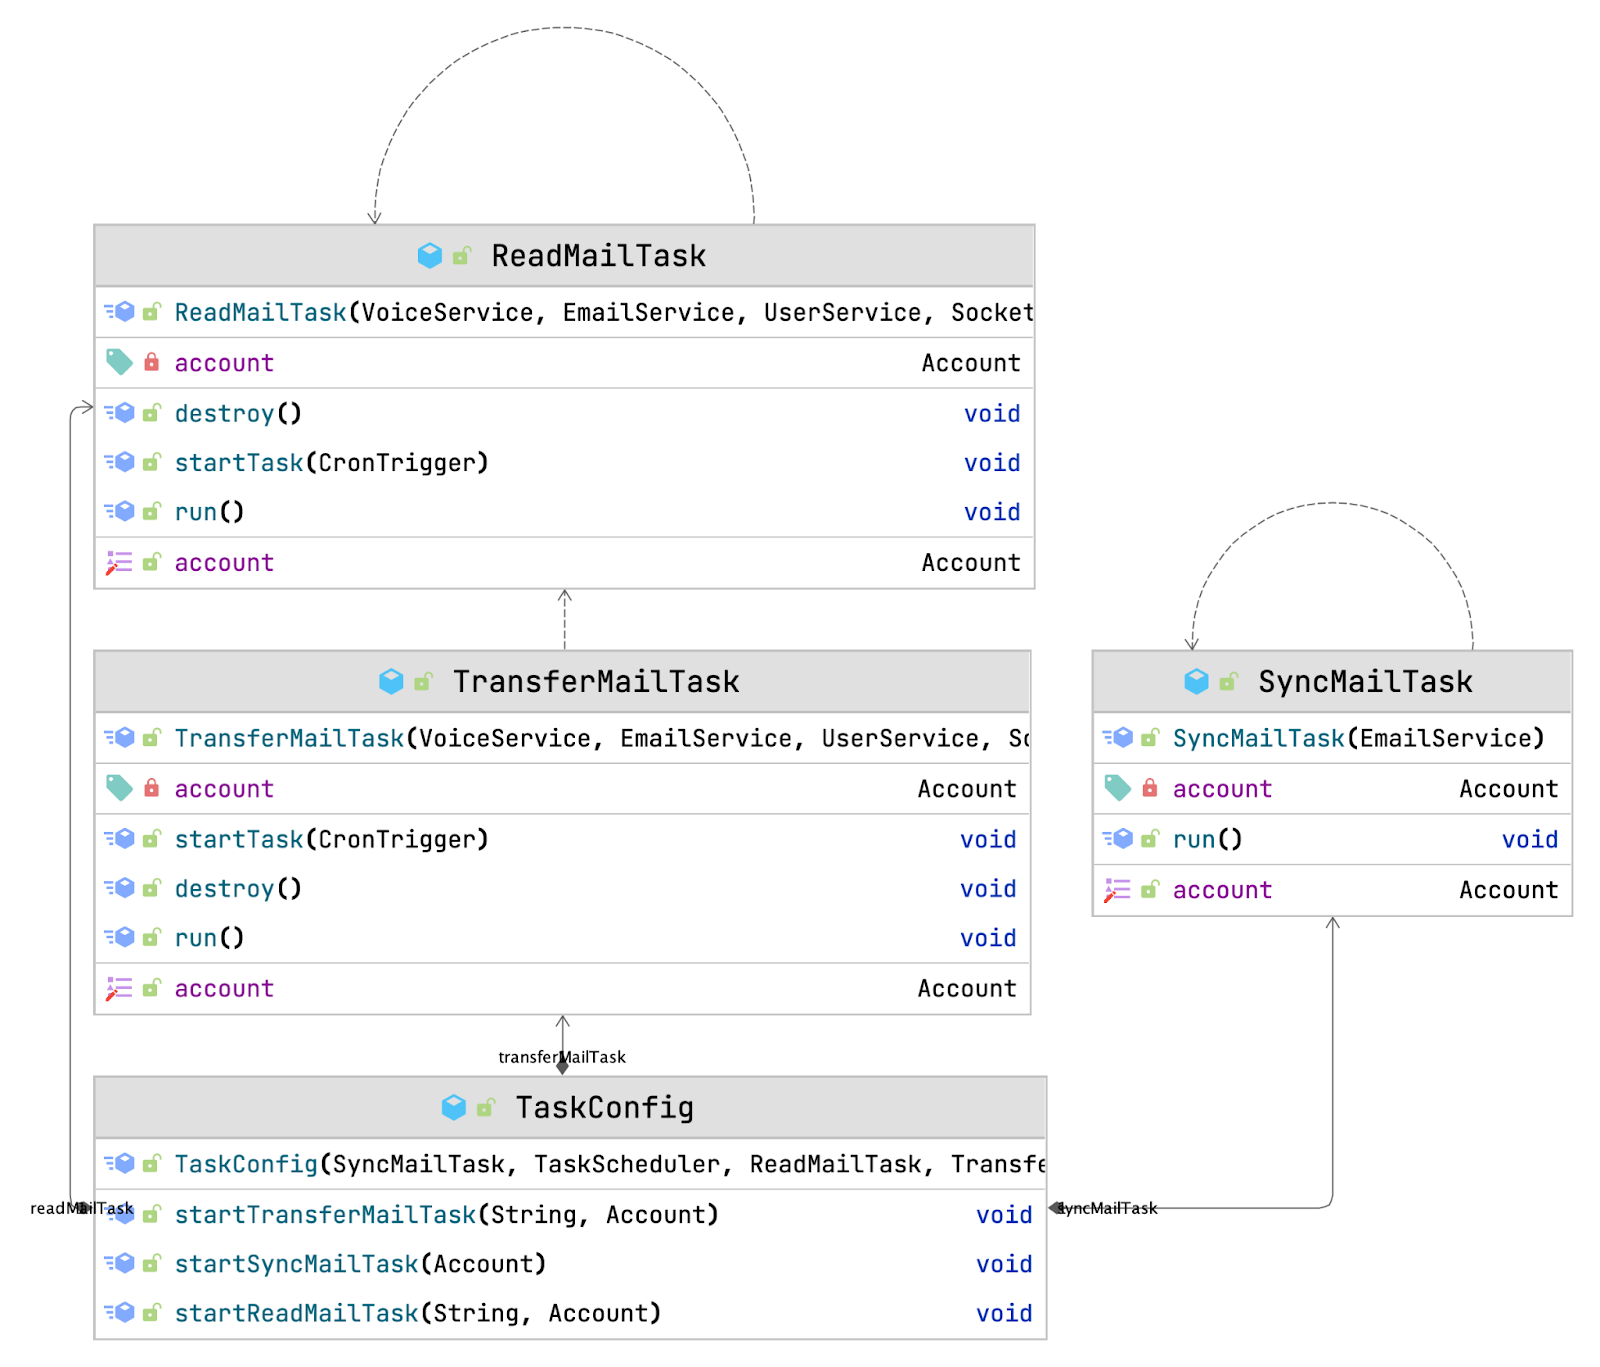
\includegraphics[width=0.6\textwidth]{scheduledTasks.png}
\end{center}
\begin{center}
Figure10: scheduledTasks
\end{center}
\subsubsection{TTS Model and TTS httpHandler}
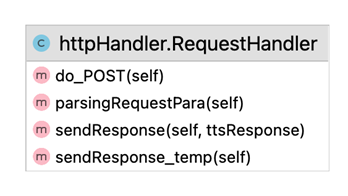
\includegraphics[width=0.3\textwidth]{httpHandler.png}
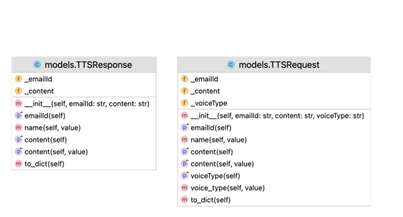
\includegraphics[width=0.5\textwidth]{TTSModel.png}
\begin{center}
Figure11: httpHandler and TTSModel
\end{center}

We use the Python script httpHandler.py (pictured above, bottom image) to allow communication and transfer of data between our TTS part (written primarily in Python) and our email part (written primarily in Java). Communication and transfer are achieved through https requests. The script contains the function ‘startServer’ and the class ‘RequestHandler’, which inherits methods and behaviours from the ‘BaseHTTPRequestHandler’ class from the Python http.server library. The class within httpHandler.py, ‘RequestHandler’, also relies on two classes imported from the team-created models.py script, which are: 
\begin{enumerate}
\item ‘TTSRequest’, for transferring data (e.g. email content) from the email part to the TTS part; 
\item ‘TTSResponse’, for transferring data (e.g. the path to the synthesised speech) from the TTS part to the email part.
\end{enumerate}

‘RequestHandler’ is executed when it is called by ‘startServer’. The class handles http requests using 3 methods, detailed below.

\texttt{ do\_Post } checks the hosts path, and if the path is correct, it gets the email id, email contents, and voice settings from the email component. It then passes these data as parameters to the ‘tts’ function and gets back a path to a wav file containing the synthesised email contents. When conversion is complete, the email id and path to the wav file are sent to the email part, using ‘TTSResponse’. If the path is not correct, then a 404 error message is thrown.

\texttt{parsingRequestPara} is called by \texttt{do\_Post} in order to get and parse the initial request from the server, after the email part has made a request to the server. It reads the request while decoding it to utf-8. It then loads the request as a json, and then uses ‘TTSRequest’ in order to return data, which are the email id, email contents, and voice settings.

\texttt{sendResponse} is also called by \texttt{do\_Post} and prepares the data from the \texttt{TTS} part to be transferred to the email component. 

\subsubsection{Frontend}
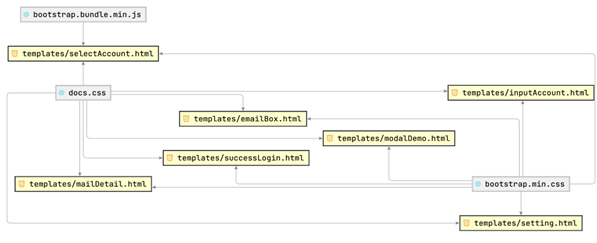
\includegraphics[width=0.8\textwidth]{FrontEnd.png}
\begin{center}
Figure12: FrontEnd
\end{center}

There are several reasons we chose Thymeleaf and Bootstrap:


Strong adaptability: Bootstrap is a popular front-end framework that provides many ready-made components and styles, making it easy to create responsive layouts that work on various devices. Thymeleaf is a popular server-side template engine that can easily render dynamic data into front-end pages.

High development efficiency: Bootstrap provides a large number of CSS and JavaScript components and plugins, enabling developers to quickly create attractive UI designs and reducing the time spent writing CSS and JavaScript. Thymeleaf is a server-side \texttt{Java} template engine that allows for seamless integration with SpringBoot. Additionally, Thymeleaf provides an intuitive way to define dynamic data and page rendering, allowing developers to focus more on implementing business logic.

Easy to learn: Both Bootstrap and Thymeleaf have extensive documentation and community support, with many examples and tutorials available to make learning and using them easier. The syntax of Thymeleaf is easy to learn and understand, and it supports both HTML and XML markup, making it a flexible option for designing web pages.

Strong extensibility: Because Bootstrap and Thymeleaf are both open-source, they can be easily extended and customized to meet the needs of different projects.

In summary, using Thymeleaf and Bootstrap can improve development efficiency, reduce the time spent writing CSS and JavaScript, create more attractive and responsive UI designs, and be easy to learn and extend.


\subsection{Database Diagram}
The \texttt{audioEmail} database schema includes several tables for managing email and user accounts. The \texttt{mail\_info} table stores information about emails, including message ID, sender, recipient, subject, content, read status, and timestamps for creation and deletion. The \texttt{mail\_file} table stores information about attachments for emails, including the filename, size, and URL. The \texttt{system\_account} table stores user account information, including the user ID, email address, password, username, and settings for SMTP, IMAP, account type, and device ID. The \texttt{device} table stores information about devices associated with user accounts, including the device ID, user ID, and device content. The \texttt{tts\_info} table stores text-to-speech information, including the ID of the associated email and the content to be read. The \texttt{account\_schedule} table stores information about scheduled text-to-speech conversions, including the ID of the associated user account, the scheduled time, and the voice type to be used. All tables include foreign keys to maintain referential integrity.


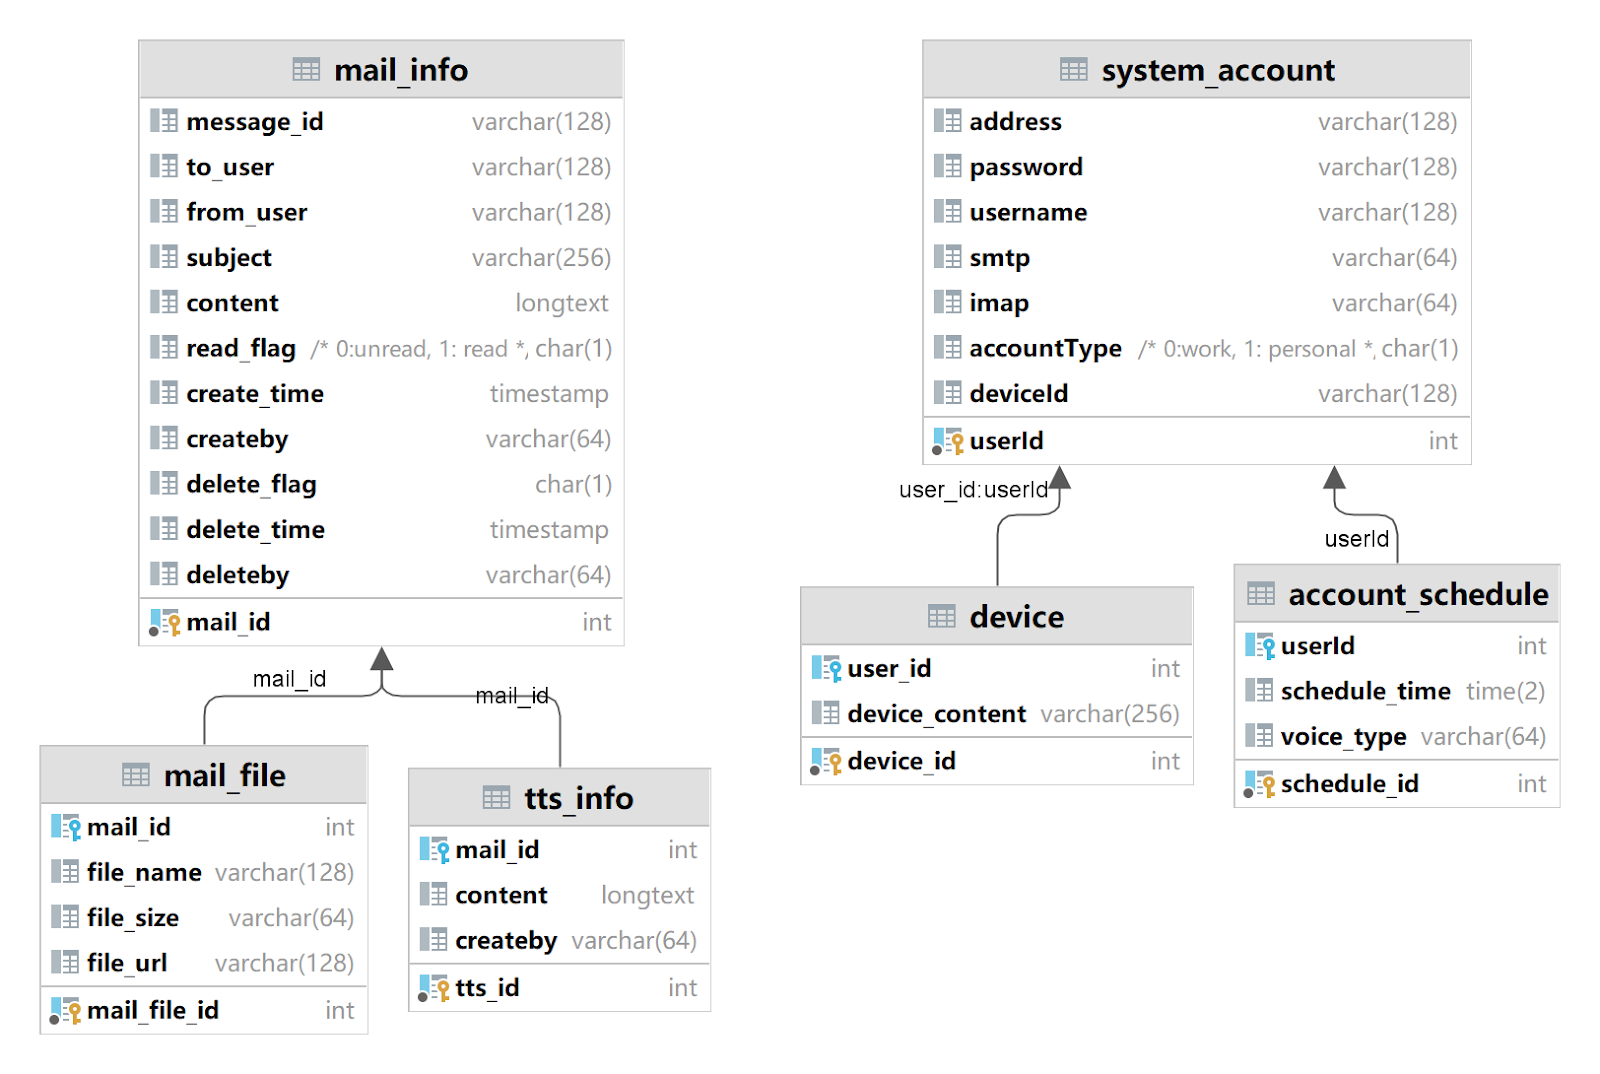
\includegraphics[width=0.8\textwidth]{DiaDatabase.png}
\begin{center}
Figure13: DiaDatabase
\end{center}


\section{Evidence of Testing - Test plan, Test Documentation and Test Results}
\subsection{Test Tools}
During the testing process, various tools can be used.
\begin{itemize}
\item SpringShell
\item JupyterNotebook
\item Python Script
\end{itemize}
At the begining, we considered using Postman for API testing and JUnit for white box testing of MailPart. However, we realised that using Postman would add an extra learning curve for team members since the inter-system call is not complex. Therefore, we decided not to use this tool.

At the same time, we encountered some strange problems while configuring JUnit. After running the test cases, we did not receive any response. After several days of trying, we were forced to abandon JUnit and use SpringShell as a temporary replacement.

Regarding TTS, testing was performed through the dedicated file \texttt{test.py}. This file imported the TTS module and from it called the tts function. The file could then be used to pass test strings. For example, in whitebox testing, we would pass different html strings that may pose varied problems (e.g. text containing foreign characters or unusual punctuation). By having unit testing specifically for the TTS part of our app, we saved time, as we did not run the entire application,

\subsection{Examples of Test Cases}
The commit record means: the commit id when the bug is fixed.
These are just some of the bugs that took us a lot of time. For other bug fixes, check the commit log in gitlab. 
When doing the white box testing, most function did not have many \texttt{if} statements, so the coverage is not a key metric for us.

\paragraph{Test case 1: Read mail}
\begin{itemize}
\item Test step: \\
    Input is ‘As an AI language model my knowledge cutoff is 2021’
\item Expected Result: \\
    The sentence above is the input content, it should read ‘2021’ as ‘twenty twenty one’
\item Test Result: \\
    It just reads ‘one’
\item Commit record: \\
    42a672e95ab3409e4913e437d138111edec408de
\end{itemize}


\paragraph{Test Case 2: Read a single email}
\begin{itemize}
\item Test step: \\
    After login, click the read button of an email
\item Expected result: \\
    User should be able to see the audio dialog box
\item Actual result: \\
    Nothing happened
\item Commit record: \\
    da95b010d6c7e8566a1cc4735f9826c568bcc04e
\end{itemize}




\paragraph{Test case 3: Wav generation time test}
\begin{itemize}
\item Test step: \\
    I sent an email that was 100 words long, to test the time taken to generate the wav file
\item Expected result: \\
    The time taken should be under one second
\item Actual result: \\
    \begin{tabular}{|l|l|l|l|} 
    \hline Content length (no. words) & Punctuation & Generation time (sec) & Wav length (sec) \\ 
    \hline 40 & NO & 10 & 30 \\
    \hline 42 & YES & 12 & 32 \\
    \hline 100 & NO & 25 & 85 \\
    \hline
    \end{tabular}
\item Commit record: \\
    42a672e95ab3409e4913e437d138111edec408de
\end{itemize}

\paragraph{Test Case 4: Common French in email}
\begin{itemize}
\item Test step: \\
    Added some common french words in an English sentence
\item Expected result: \\
    Read all of the words or skip any unknown words
\item Actual result: \\
    French letters caused TTS part to throw errors
\item Commit record: \\
    42a672e95ab3409e4913e437d138111edec408de
\end{itemize}

\textbf{More test cases can be found in the Appendix.}



\section{Team management \& communication}

\paragraph{Organisation of the team and use of tools:}\hspace{0pt}\\
Each of us is an active team member and project builder, however, we also adopted specific roles. For example, while Mingqing, Nana and Ziyu primarily worked on the email part, Baiyang, Georgia and Hok Yan primarily worked on the TTS part. We spent the first week organising the team and defining the roles and responsibilities of each member before we started the technical part of the project. We set reminders for each important time point and then planned all tasks for each phase. Our model for carrying out the project was to meet twice a week to plan and summarise, and to discuss and resolve any issues we were encountering. Each member allocated several hours outside of the meetings to work on programming. 

In the second week, once we met our team members, we wrote our team operating agreement. This document defined how to manage our team and communicate for the rest of the project. The latest version of this document is available from our Google Drive, the link to which is in the Appendix. We assigned specific members to work on each task (e.g. on Trello). However, members were also free to assist on a task they were not assigned to. 

\paragraph{How the team communicated throughout the project:}\hspace{0pt}\\
We held bi-weekly meetings, which were attended by all members. In the few cases where not all members were able to meet in person, members were able to attend remotely using Google Meet. These bi-weekly meetings were the Tuesday lab session, and an additional team meeting every Thursday. The main purpose of the Thursday meeting was to pair-program, resolve any issues that team members had encountered and push code to GitLab. In preparation for the client meetings, we held additional meetings on Monday evenings in Weeks 8 and 11. 

During meetings, Georgia acted as facilitator and checked everyone's progress. We then defined our respective tasks before the next meeting. We kept minutes of the meetings, an excerpt of which is presented in the communication section. Outside of meetings, we used a group chat on the online messaging platform 'Whatsapp' to provide support in a timely manner and give each other quick updates. We also used this chat to vote on decisions, using the Whatsapp ‘poll’ function. For example, we used a Whatsapp poll to vote on whether we should take a break over the Spring holiday or we should treat the Spring holiday as another sprint. We voted unanimously in favour of the latter. We used Miro for user stories and Trello for backlog to track tasks and progress.

All code and README files were shared via Gitlab. We also had a Google drive specific to the team project for formal communications: meeting agendas and minutes; specifications; and notes of issues to be raised with the advisor.

During the course of the project, members who were more familiar with a given area would support other members. For example, Mingqing created and shared JSON.md and JSON.pdf to aid his teammates' understanding of \texttt{json} objects and how they can be used to transfer data. These files can be accessed on our Google drive.

\subsection{Management}
\begin{itemize}
    \item Team Collaboration
    \begin{itemize}
        \item Georgia is responsible for team coordination and communication, moderates meetings, and organises documents.
        \item Hok Yan Pun is responsible for arranging meeting locations and editing documents.
    \end{itemize}
    \item System Design
    \begin{itemize}
        \item UI and function Design
        \begin{itemize}
            \item All team members participated in this part.
        \end{itemize}
        \item Research on SMTP and IMAP (Nana)
        \item Research on TTS API (Baiyang)
        \item Research on hashing password (Georgia)
        \item Database Design (Ziyu; Baiyang)
    \end{itemize}
    \item System Development
    \begin{itemize}
        \item TTS
        \begin{itemize}
            \item Text processing (Hok Yan)
            \item Speech synthesis (Georgia)
            \item Connector to Email (Georgia; Mingqing)
        \end{itemize}
        \item Mail Part
        \begin{itemize}
            \item Backend
            \begin{itemize}
                \item Login (Ziyu; Mingiqng)
                \item Scheduled Task (Mingiqng; Ziyu)
                \item Send/Receive Mail (Mingqing; Ziyu; Baiyang)
                \item Handlers of IMAP/SMTP (Nana; Mingqing)
                \item Settings (Ziyu; Mingqing)
                \item Connector to TTS (Mingqing; Georgia)
            \end{itemize}
            \item Frontend
            \begin{itemize}
                \item Login (Ziyu; Hok Yan; Nana)
                \item Inbox (Ziyu; Nana; Hok Yan)
                \item Setting (Ziyu; Mingqing; Hok Yan)
            \end{itemize}
        \end{itemize}
    \end{itemize}
    \item System Testing
    \begin{itemize}
        \item White Box Test
        \begin{itemize}
            \item TTS (Georgia)
            \item Email (Baiyang)
        \end{itemize}
        \item Black Box Test
        \begin{itemize}
            \item Email (Nana)
        \end{itemize}
        \item Bug Fix
    \end{itemize}
    \item Final Report (All team members participated in this part.)
\end{itemize}
\includegraphics[width=1\textwidth]{GanttChart.png} \\
\begin{center}
Figure14: GanttChart
\end{center}
\\
The above is the overall task management of the project, which was mostly unchanged from the beginning of the project. Mingqing, Ziyu and Nana focused on the email functionality from the start, and Georgia, Baiyang and Hok Yan on TTS. As certain sub-tasks were completed, Baiyang joined the email back-end, and Nana and Hok Yan moved onto the front-end; while Georgia was responsible for implementing the new speech synthesis strategy, and Mingqing and Ziyu remained the pillars of the email back-end. As some members were not familiar with git, certain functionalities were developed, tested and debugged mostly on local drives, with occasional commits to GitLab that included multiple fixes.


Minutes usually followed this structure: 
\begin{itemize}
    \item  each member summarised what they had been working on in the past week; 
    \item  we would take note of any reminders to ourselves that resulted from our discussions; 
    \item each member updated the team on what they planned to work on next. This helped us to avoid multiple people working on the same task, and thus saved us time.
\end{itemize}

There have been no major disagreements in the team. When issues arose, we discussed together as a team, considering the practicalities of the project; each member's abilities; and considered the client requirements to reach consensus. If discussion did not reach consensus, we used polls, as mentioned above. In the case of miscommunication, we all tried to be understanding and just focused on solving the problem at hand.

\section{Planned \& Completed Features}
This section presents the user stories that were planned and completed in each sprint. All of the features listed in PROJECT REQUIREMENT FORM are completed. We have also completed a number of extra functions to improve user experience.
\begin{itemize}
    \item Week2
    \begin{itemize}
        \item List user stories
        \item Feasibility analysis (SMTP/SPAM)
    \end{itemize}
    \item Week3
    \begin{itemize}
        \item Learn git
        \item Build development environment
        \item UI Design
    \end{itemize}
    \item  Week4 
    \begin{itemize}
        \item Use case diagrams
        \item Sequence diagrams
        \item User story mapping
        \item The priority of the user stories
        \item How to handle HTML
    \end{itemize}
    \item Week5
    \begin{itemize}
        \item Build connector between Java and Python
        \item EmailService
    \end{itemize}
    \item Week6 
    \begin{itemize}
        \item Check if we have the basic functionality ready, and then decide which non-essential features to work on first
        \item Login functionality
        \item Basic text processing
        \item Basic speech synthesis
    \end{itemize}
    \item Week7
    \begin{itemize}
        \item Send and receive mails
        \item Research how to speed up TTS
        \item Put together prototype for TTS
    \end{itemize}
    \item Week8
    \begin{itemize}
        \item Bug fix
        \item Scheduled Task
        \item Use socket to send resource path
    \end{itemize}
    \item Week9
    \begin{itemize}
        \item Voice list 
        \item System Test
    \end{itemize}
    \item Week10
    \begin{itemize}
        \item Bug fix 
        \item Upgrade UI
    \end{itemize}
    \item Week11
    \begin{itemize}
        \item Display a prompt when the software throws an exception
    \end{itemize}
\end{itemize}

\section{Extra Completed Features}
\begin{itemize}
    \item More voice options \\ 
    The requirement asked for 2-3 kinds of voice, we offer 7 different accents to provide greater choice.
    \item Account delete \\ 
    We added an account deletion button on the login page to delete accounts that are no longer needed.
    \item Sync function \\ 
    On the inbox page, there is a sync button in the top right corner that can be used to sync emails received in real time. Syncing also be uploads data to our database.
    \item Emails delete \\ 
    Users can indicate one or more emails to delete on the inbox page.
\end{itemize}

\section{Uncompleted Features}
This section is about the features that were not completed and the reasons why.
\begin{itemize}
    \item Password hashing \\ 
    Initially we hashed the user's password, but then we discovered that the App password used by the IMAP protocol had to be a cleartext password when we fetched the user's email message via IMAP.
    \item Clearly distinguish between read and unread. \\ 
    The project uses an additional column to the email list to differentiate the read/unread status of the emails. This approach may not be as visually clear as other email clients (e.g. Google Mail uses different background colours to distinguish read/unread). The reason for this is that we lacked sufficient time to research design.
    \item  Display conversion progress \\ 
    There is no indication of text-to-speech conversion under progress, so the user would not know what is happening with the program if the conversion takes too long. This problem was not foreseen in the design stage.

\end{itemize}


\section{Conclusion}
\subsection{What we have learned}

The following summarises the knowledge we have gained through this project:

The importance of teamwork: We were able to successfully complete the project through communication, co-ordination and support. We learnt how to collaborate as a team, how to distribute tasks, and how best to support others in the team.

Technical skills enhancement: In this project we used a variety of techniques and tools, such as productivity managers (e.g. Trello) and software libraries/engines (e.g. NLTK, Thymeleaf). This has expanded our skill-set and sharpened our problem-solving skill. We have also learnt how to write better, more readable code and how to conduct code reviews.

The importance of project management and planning: We learned how to set clear objectives and deadlines, as well as how to track progress and manage risks. We learned to change tactic if required by the client. For example, we changed the speech synthesis technique in order for the speech to have improved quality.

\subsection{Challenges we have faced and resolved}

We also encountered some challenges in this projects. One of these issues was the diversified team background. Everyone in the team has a different academic background. For example, two members had an undergraduate background in linguistics and one in Electronic Information Engineering. Among the other three members, one member had more experience with C++ but lacked web development experience, while the other two had more Java development experience.

Our corresponding solution was:

 To maximise the development efficiency, we decided that three members (Baiyang, Georgia and Hok Yan) would be responsible for TTS based on Python, as they were taking the Speech and Language Processing program, and they all had a foundation in Python. The three remaining members, on the Advanced Computer Science program would be responsible for web development and design. Since these members did not all take the IntelligentWeb course and were not particularly proficient in Javascript and Nodejs, we ultimately decided to use Java for the development. Additionally, during the system design and requirements analysis phase, this diverse background provided us with great help, and each person put forward valuable opinions on the system's functionality and design.

Another problem was that we initially underestimated the complexity of the project. We believed that three people each could develop the TTS and email parts, respectively, and still meet our schedule. As a result, in the early stages of the project, only one or two members built the entire Java and Python development environment, independently of one another. Our underestimation of the project's complexity also led to the fact that we did not set up a clear and specific testing plan. Therefore, it was not until later in the development process that we started to spend more time on testing. Additionally, during the initial testing process, we relied on the more experienced members of the team to test the features they developed. However, developers may have a bias towards their own code and may overlook certain defects or issues. Having separate testers would have ensured that there was an unbiased evaluation of the code.


Initially, we adopted concatenation to generate the audio, and the text processing was done on a granular level to account for the complexity of language/text in email content. After discussing with the client, the audio quality produced by this method was decided to be unsatisfactory, so we searched for alternative methods. We ultimately decided on the gTTS library for TTS. This library produces higher quality speech than our previous method. However, in isolation, the gTTS library could not address all of our text-preprocessing and speech synthesis needs (Sections 5.3.1 and 5.3.2). Therefore, our final strategy was to combine the gTTS library with our previous text-preprocessing code as well as some speech post-processing on the phrase-level. 

Overall, we learned how to collaborate, and manage and plan projects. We improved our technical skills and learned how to problem solve. We learned the importance of planning, and that lack of planning in one aspect will lead to later problems. For example, we began the testing process later than was ideal.

\newpage
\section{Appendix}

\subsection{User guide}

\underline{Subsequent log-ins (after set-up):}
\begin{enumerate}
  \item Open the localhost:8083/audioEmail/login/loading/
  \item You will see the webpage pictured below \\
  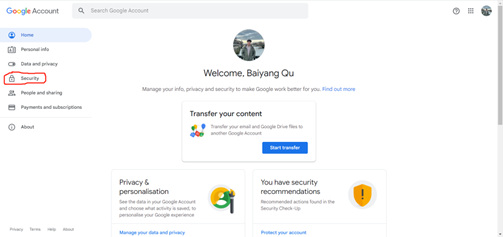
\includegraphics[]{google security.png} \\
  \item Input email address, e.g. ‘crowds723@gmail.com’
  \item Input password, e.g.  ‘omitted’
  \item Choose account type, between ‘personal’ and ‘work’
\end{enumerate}

\noindent \underline{Log out and log in with another account:}
\begin{enumerate}
  \item Click 'log out' on the left hand side, you will be taken to the login page shown above
  \item Input email address and password
  \item Choose account type
\end{enumerate}

\noindent \underline{Send Mail between work and personal account (two accounts in two browsers):}
\begin{enumerate}
  \item Open two web pages in order to log in to your accounts
  \item In one account click 'Write Message' on the left hand side, write the recipient, subject and body, and then send
  \item In the other account, click Sync, or logout and login again - you should see the email from the other account in your inbox
\end{enumerate}

\noindent \underline{Reading emails, or having emails read to you:}
\begin{enumerate}
  \item Navigate to your inbox, you should see a list of emails
  \item Under the 'Operation' column, you should see two buttons for each email: 'Read' and 'Detail'
  \item To view email text, click 'Detail', this will take you to a different page that contains the email content as text
  \item To have the email read to you, click 'Read', this will open a playable window on the inbox page. Clicking the play button (the arrow icon) should begin playback, and you should hear speech
  \item Volume can be adjusted by clicking the loudspeaker icon and dragging the slider up or down
\end{enumerate}

\noindent \underline{Change settings:}
\begin{enumerate}
  \item Navigate to the settings menu, on the left hand side
  \item From here you can change username, email address, voice type (accent), and you can set a scheduling time
  \item After adjusting settings, click 'Save' to keep your changes, or 'Reset' to return to the default settings
\end{enumerate}

\noindent \underline{Set scheduling time:}
\begin{enumerate}
  \item Follow step 1 in 'Change settings'
  \item In the drop down menu titled 'Schedule Time', choose the time that you want the application to start reading emails
  \item Save and exit the settings page
  \item To hear playback at your selected time, you will need to have logged into your account by the selected time
  \item (Please note that selecting all unread emails to be read uses similar functionality, however, playback may take longer to begin)
\end{enumerate}

\pagebreak
\subsection{Setup Guide}
This guide applies for all operating systems. The script ‘dependencyHandler.py’ must be executed by the user. It checks the system for the necessary imports, and then installs any missing dependencies.
\begin{enumerate}
\item How to get the app password
    \begin{description}
        First time login: The user will need to get an ‘App password’ from Google. Instructions may differ slightly if the user does not have a Google account. However, the user can search for ‘App Password’ from the homepage of their email provider.
    \end{description}
    \begin{itemize}
        \item Navigate to Google account. The web address should start with ‘https://myaccount.google.com/’.
        \item If not enabled, enable 2-step Verification, which can be found on the Security page under the heading ‘How you sign in to Google’.
        \begin{itemize}
            \item  Google Account $\rightarrow$  Manage Accounts
            \begin{center}
                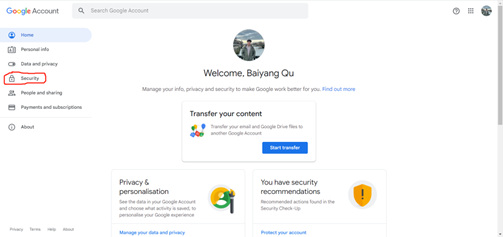
\includegraphics[]{google security.png}
            \end{center}
        \end{itemize}
        \item Once you click ‘TURN ON’ on the 2-step Verification, you will be prompted to enter your mobile phone number, with the choice of receiving either a voice or text message.
        \item Follow the instructions and enter the verification code by whatever means you selected in the previous step.
        \item Navigate back to the Google account homepage.
        \item Search for ‘App Passwords’, and a suggestion with the same name should appear under ‘Security’. Click this suggestion.
        \begin{center}
            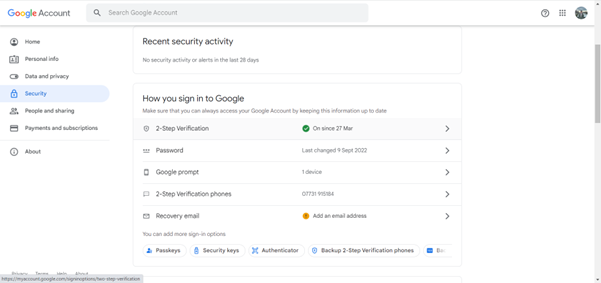
\includegraphics[]{google verfication.png}
        \end{center}
        \begin{itemize}
            \item You will see two drop-down menus called ‘Select app’ and ‘Select device’. Under ‘Select app’, you must select ‘mail’. Under ‘Select device’ you should select the device on which you wish to use MyAudioEmailr. For example, if you want to open MyAudioEmailr on an iPhone, then you should select ‘iPhone’.
            \item Once you click ‘GENERATE’, you will be given an app password. You can now continue following the steps below.
            \begin{center}
                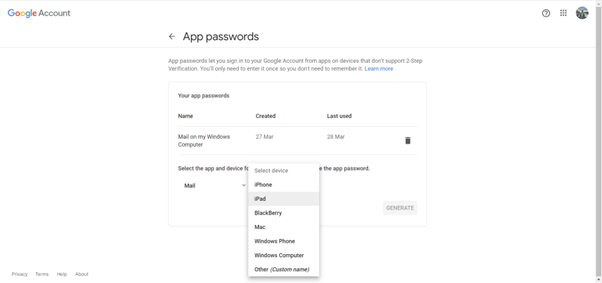
\includegraphics[]{app password.png}
                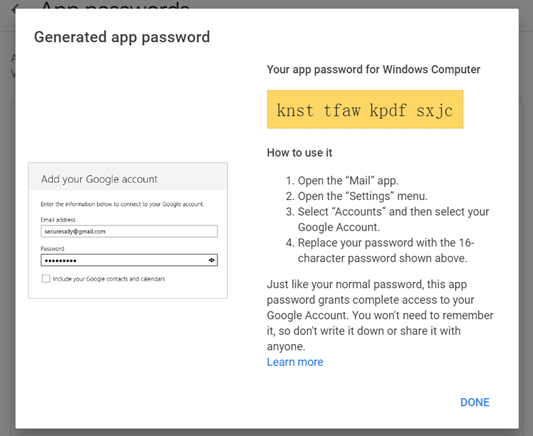
\includegraphics[]{generate password.png}
            \end{center}
        \end{itemize}
    \end{itemize}
\item Python files for deployment on the server
\item Pip install packages
\item Run python script
\item Configuring the database
\item You need to configure the application.properties file, which including the file path and the database address
\begin{center}
    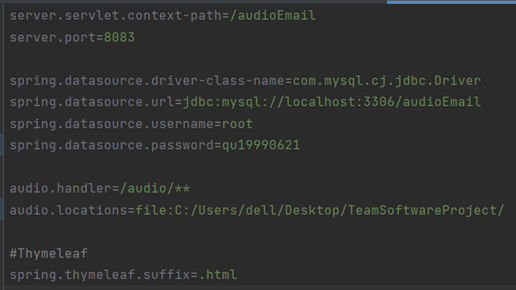
\includegraphics[]{application properties.png}
\end{center}
\item Build the project into a jar package
\item Deploy the jar package on the server (linux) and use the bash script to start the jar package.
\item Or run the email part via Intellij directly(without building and deploying)
\item Open a browser to access the project address.
    \begin{center}
        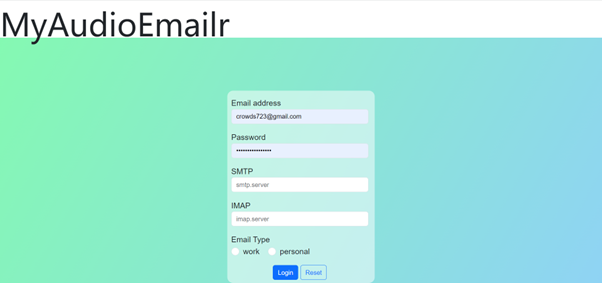
\includegraphics[]{User Guide login page.png}
    \end{center}
\end{enumerate}
\subsection{Class Diagram}
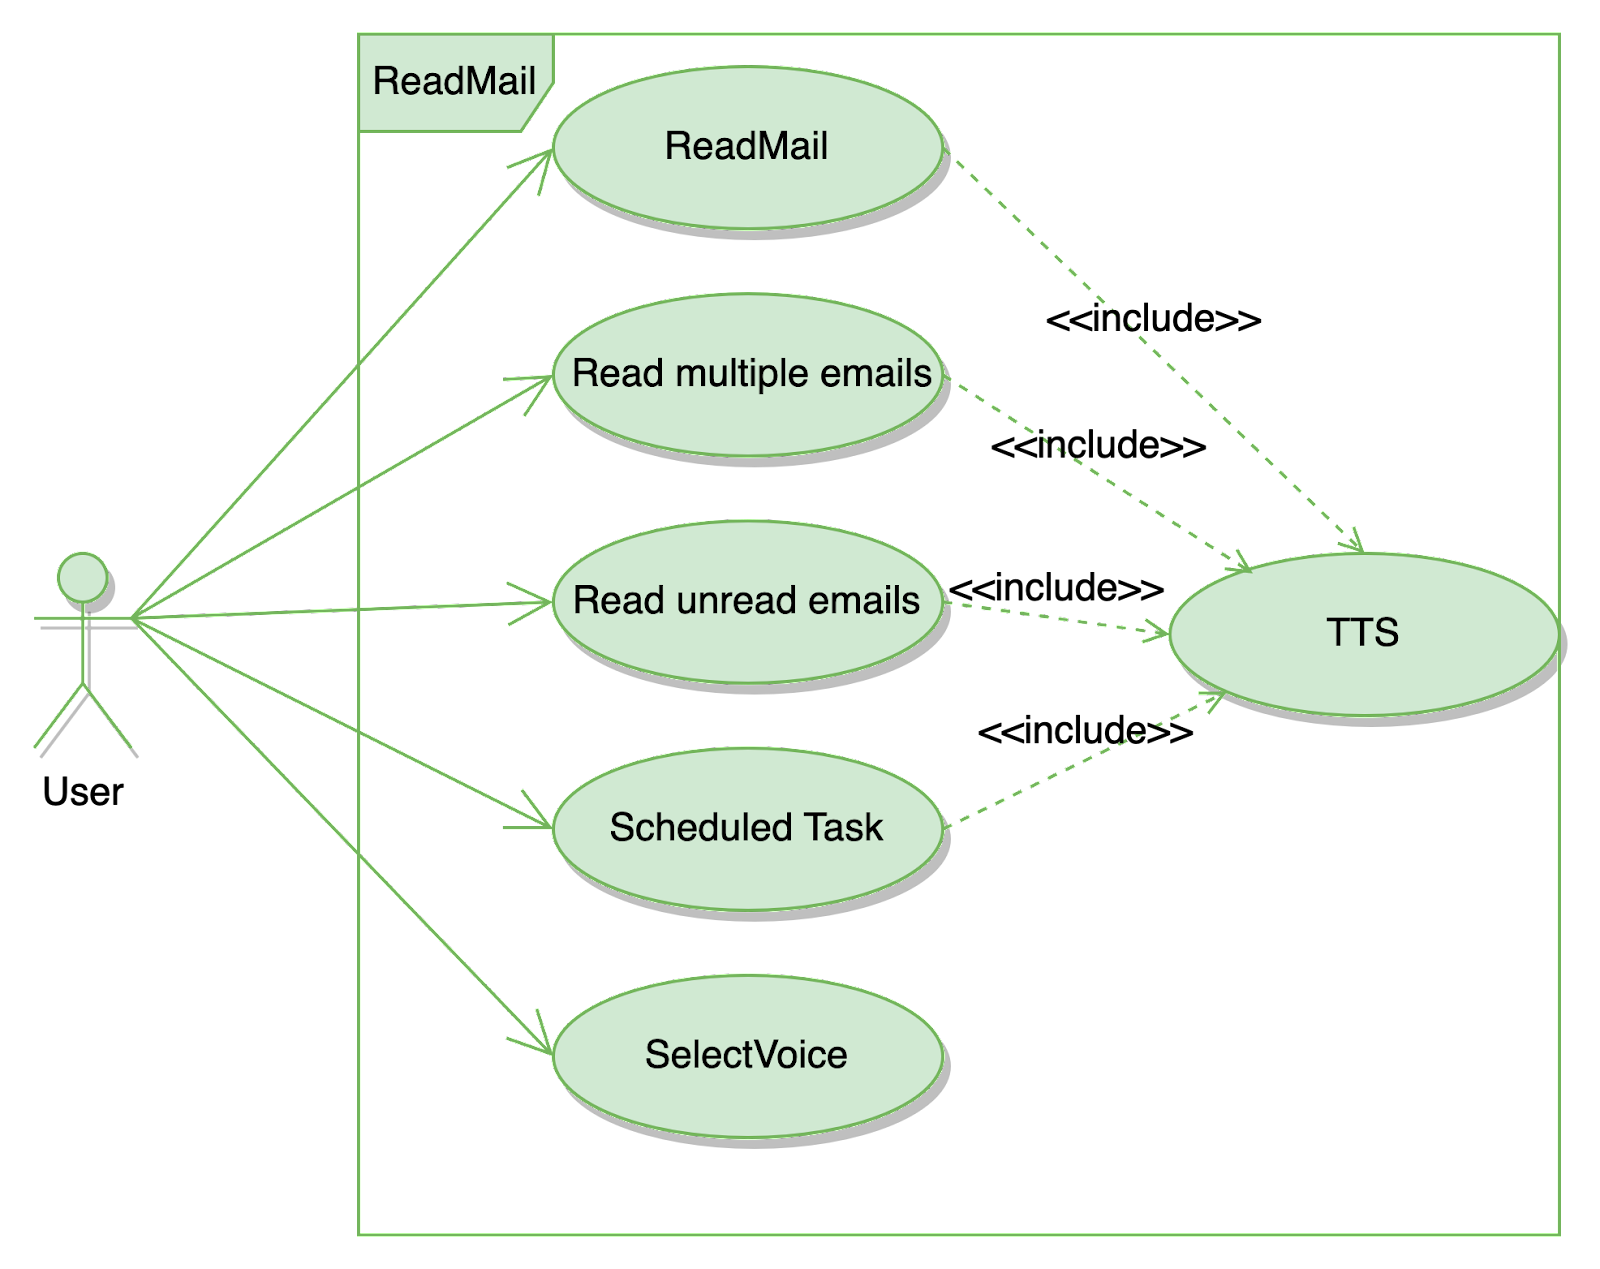
\includegraphics[width=0.8\textwidth]{UserCase_ReadMail.png} \\
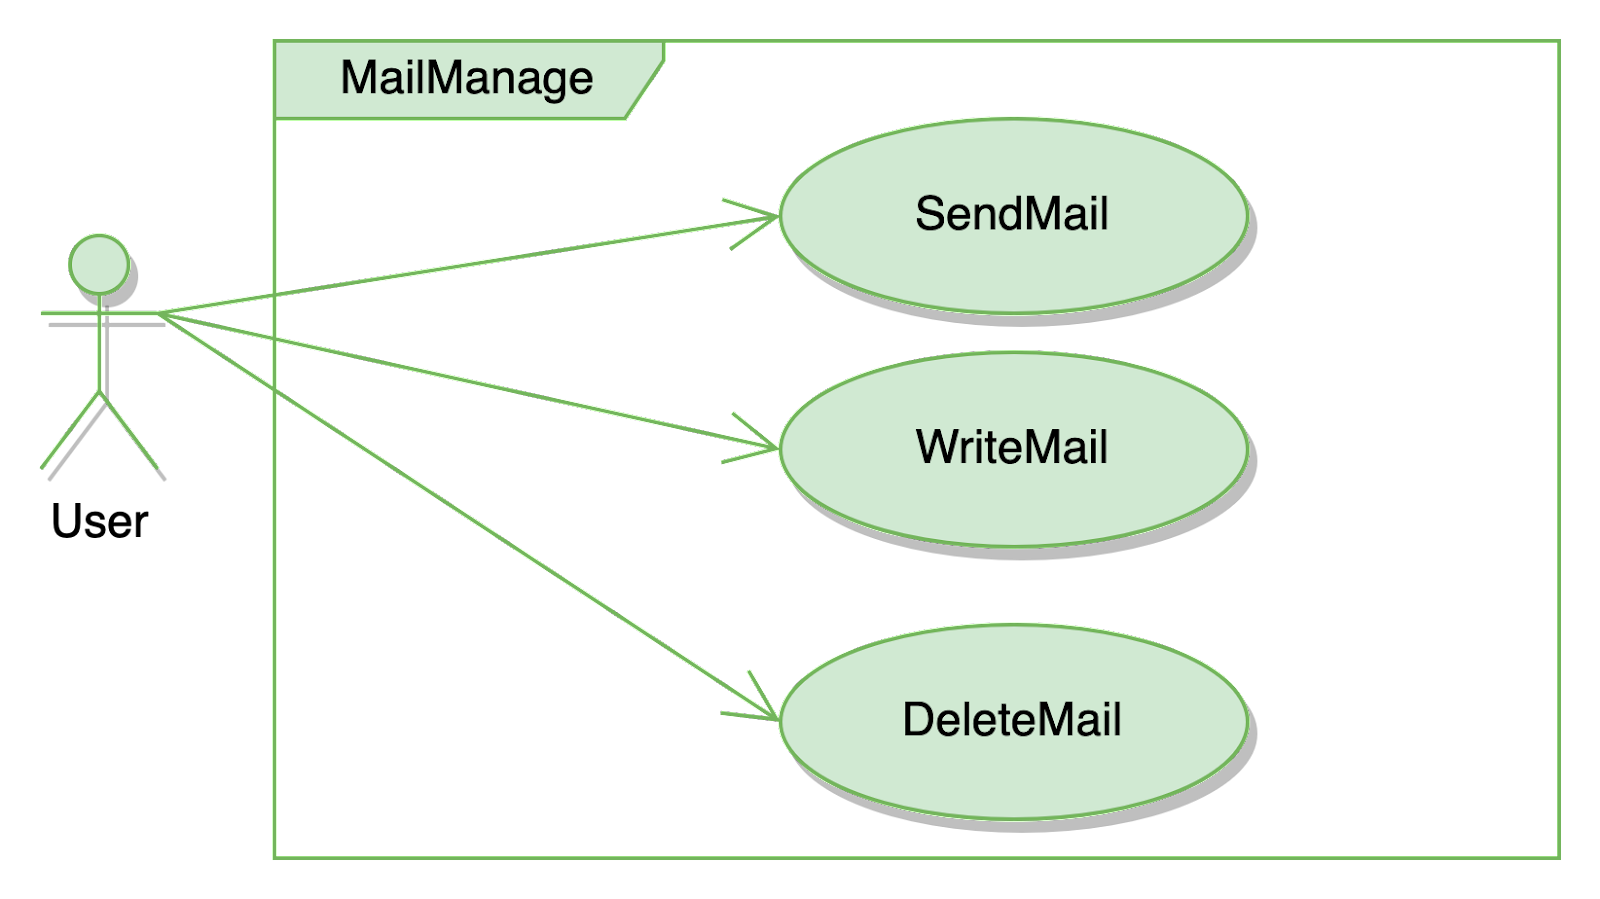
\includegraphics[width=0.8\textwidth]{UserCase_MailManage.png}
\subsection{Minutes for week3}
\paragraph{Meeting on Thursday 23/02/2023 at 11:30
And ended around 12:45
} \hspace{0pt}\\
This week: \\
\begin{itemize}
    \item Mingqing is working on git lab and writing documentation about the software we will write. He will share it with the group later.
    \item Ziyu is designing the database structure (MySQL). Ziyu and Mingqing are planning to work on the back end.
    \item Baiyang is supporting Ziyu and is learning MySQL.
    \item Rachel will go through the agenda - she has watched the pre-recorded content and made notes on it (shared in WhatsApp group). Rachel has suggested a collaborative agenda and she would like to be in charge of editing the agenda.
    \item Nana is working on the spec end with Mingqing and Ziyu.
    \item Georgia is researching TTS..
\end{itemize} \\
General points: \\

\begin{itemize}
    \item Division: 3-3 split - Nana, Mingqing, Ziyu on more technical parts (database and Java). Baiyang, Rachel and Georgia on TTS.
    \item We will store all documentation on Google Documents.
    \item Everyone should have their own branch on Git Lab. Use of Git Lab off-campus requires a VPN.
    \item Okay to use Word, but it is common practice to use markdown or LaTeX.
\end{itemize} \\

Next week: \\

\begin{itemize}
    \item Mingqing and Nana are going to work on the sending and receiving email functionality.
    \item Ziyu will work on building the environment
    \item Baiyang, Rachel and Georgia will work on the TTS function. It will be written in Python. We need data: diphones, any open-source set, prosody and word sense disambiguation possibly from NLTK. Baiyang will work on the schematic while Georgia and Rachel will work on gathering data.
    \item On Tuesday we will talk about the key features. We will clarify with Ola regarding preferred language.
\end{itemize}
\subsection{Additional test cases}

\subsubsection{Test Case 5: Unread email state}

\paragraph{Test Case 5: Unread email state}
\begin{itemize}
\item Test step: \\
    ASend a new email
\item Expected result: \\
    The email should be marked as unread before opening or reading it 
\item Actual result: \\
    The email is marked as read once user receives it
\item Commit record: \\
    1568f9379e775d4ce0e79ae1d60613de43993be6
\end{itemize}

\subsubsection{Test Case 6: send email}
\paragraph{Test Case 6: send email}
\begin{itemize}
\item Test step: \\
    Try to send an email via the ‘write message’ button
\item Expected result: \\
    Receive the email in the account specified in ‘recipients’
\item Actual result: \\
    It shows ‘send failure’ first, but I can get the email sent to my personal account
\item Commit record: \\
    061c97a4000c19264807d8a924efc49b7fa5b4d0
\end{itemize}

\subsubsection{Test Case 7: testChangeStatus}
\paragraph{TestCase 7: testChangeStatus}
\begin{itemize}
\item Test intput: \\
    \begin{lstlisting}[language=Java]
    Test Input:
    String name = "mq";
    String senderAddress = "crowds723@gmail.com";
    String receiverAddress = "mzhang122@sheffield.ac.uk";
    String smtp = "smtp.gmail.com";
    String imap = "imap.gmail.com";
    String deviceId = "202303281710-diive";
    \end{lstlisting}
\item Expected result: \\
    The status of all emails in this account should be changed
\item Actual result: \\
    Test case pass
\end{itemize}

\subsubsection{Test Case 8: testInitEmails}
\paragraph{Test Case 8: testInitEmails}
\begin{itemize}
\item Test intput: \\
    \begin{lstlisting}[language=Java]
    Test Input:
    String name = "mq";
    String senderAddress = "crowds723@gmail.com";
    String receiverAddress = "mzhang122@sheffield.ac.uk";
    String smtp = "smtp.gmail.com";
    String imap = "imap.gmail.com";
    String deviceId = "202303281710-diive";
    \end{lstlisting}
\item Expected result: \\
    The user's information is inserted into the system\_account table, and the last ten emails received are inserted into the mail\_info table
\item Actual result: \\
    Test case pass
\end{itemize}

\subsubsection{Test Case 9: syncTest}
\paragraph{TestCase 9: syncTest}
\begin{itemize}
\item  Test steps: \\
    Send an email to the currently logged in user \\
    Wait 10 mins  then check if there is a new mail in the database
\item Test intput: \\
    \begin{lstlisting}[language=Java]
    Test Input:
    String name = "mq";
    String senderAddress = "crowds723@gmail.com";
    String receiverAddress = "mzhang122@sheffield.ac.uk";
    String smtp = "smtp.gmail.com";
    String imap = "imap.gmail.com";
    String deviceId = "202303281710-diive";
    \end{lstlisting}
\item Expected result: \\
    The user's information is inserted into the system\_account table, and the last ten emails received are inserted into the mail\_info table
\item Actual result: \\
    Several emails appear, but not the latest from the database
\item Commit record: \\
    54619c53bb993dcb22822202dd3d5bcfb9a235c7
\end{itemize}

\subsubsection{Test Case 10:  playUnreadMail}
\paragraph{Test Case 10:  playUnreadMail}
\begin{itemize}
\item Test step: \\
    After login click the playUnreadMails button
\item Expected result: \\
    Users do not need to wait for all audio transcriptions to be completed \\
    All unread mails can be read one by one
\item Actual result: \\
    Users need to wait for all emails to finish processing before any are read
\item Commit record: \\
    0a1e8daffc97e55efb02339785b5393123ecff28 
    0295890ef4a22bcc470cc68acf12439a300b7e8f
\end{itemize}


\subsubsection{Test Case 11:   playSpecificMail}
\paragraph{Test Case 11:   playSpecificMail}
\begin{itemize}
\item Test step: \\
    After login click the playSpecificMails button
\item Expected result: \\
    Users do not need to wait for all audio transcriptions to be completed \\ 
    All unread mails can be read one by one
\item Actual result: \\
    Users need to wait for all emails to finish processing before any are read
\item Commit record: \\
    0a1e8daffc97e55efb02339785b5393123ecff28 
    0295890ef4a22bcc470cc68acf12439a300b7e8f
\end{itemize}

Test Case 13: Increased volume from exclamation marks
Test step:

Expected result:

Actual result:




\subsubsection{Test Case 12: Handling punctuation}
\paragraph{Test Case 12: Handling punctuation}
\begin{itemize}
\item Test step: \\
    Passed an html string containing punctuation not handled by text\_preprocessing.py (e.g. \{ or \@), with some punctuation in a sequence (e.g. ???), to tts using the test.py module
\item Expected result: \\
    These punctuation marks should be pronounced (e.g. “curly bracket”) or omitted
\item Actual result: \\
    A given punctuation mark is passed to the gTTS class as a phrase, raising an AssertionError, due to there being nothing pronounceable
\item Commit record: \\
    f9240803a42d9fd44e4615265be527d7ebc3f4fb
    eb4170f9bd747d788f9a44bce71b10e60bf15cfd
\end{itemize}

\subsubsection{Test Case 13: Increased volume from exclamation marks}
\paragraph{Test Case 13: Increased volume from exclamation marks}
\begin{itemize}
\item Test step: \\
    Using test.py, I passed a string containing some exclamation marks to tts
\item Expected result: \\
    These punctuation marks should be pronounced (e.g. “curly bracket”) or omitted
\item Actual result: \\
    Test case pass
\end{itemize}



\subsection{References}
\begin{itemize}
    \item \href{https://www.crummy.com/software/BeautifulSoup/}{Beautiful Soup 4.12.2 [software]. Leonard Richardson. (2007)}\\Accessed 10 May 2023
    \item \href{https://gtts.readthedocs.io/_/downloads/en/v2.1.1/pdf/}{gTTS 2.3.2 [software]. Pierre-Nick Durette. (2020)}
    \\Accessed 4 May 2023
    \item \href{https://ieeexplore.ieee.org/abstract/document/7829407}{Meyer, A. N., Barton, L. E., Murphy, G. C., Zimmermann, T., \& Fritz, T. (2017). The work life of developers: Activities, switches and perceived productivity. IEEE Transactions on Software Engineering, 43(12), 1178-1193} \\
    Accessed 10 May 2023
    \item \href{https://www.nltk.org/index.html}{NLTK 3.8.1 [software]. (2023)}\\ 
    Accessed 4 May 2023
    \item \href{https://www.jetbrains.com/pycharm/}{Pycharm Professional 2022.3.2 [software]. JetBrains. (2022)}
    \\ Accessed 10 May 2023
    \item \href{https://pysoundfile.readthedocs.io/en/latest/}{Soundfile 0.12.1 [software]. Bastian Bechtold. (2020)} \\
    Accessed 10 May 2023
\end{itemize}


\end{document}